% =====================================================================
%  SECTION 5 — Amortization: certificates for unseen microstructures
%  Draft 1. Every number traceable to RESULTS.md.
% =====================================================================

\section{Amortization: certificates at inference cost}
\label{sec:amortized}

Sections~\ref{sec:admissible}--\ref{sec:exact} produce a certified interval
for \emph{one} microstructure at the cost of one training run. That is the
setting of all existing variational-certificate work, neural or classical:
Gaynutdinova et al.~\cite{Gaynutdinova2026} train one network per
representative cell, and the classical schemes
of~\cite{Gaynutdinova2023} solve one linear system per
cell. For screening, design or uncertainty propagation, the settings in which many-query cost dominates, this is the wrong cost model.

This section removes the per-instance restriction. We condition the trial
fields on the microstructure so that a single trained operator emits
certified bounds for microstructures it has never seen, at inference cost.
The central observation is that this changes nothing about validity:

\begin{proposition}[Certificates survive conditioning]
\label{prop:amortized}
Let $\chi(\,\cdot\,;m)$ and $\psi(\,\cdot\,;m)$ be trial fields
conditioned on a microstructure descriptor $m$, and suppose that for every
fixed $m$ they remain $Y$-periodic and conforming in the sense of
Section~\ref{sec:admissible}. Then the bounds of
Theorems~\ref{thm:primal}--\ref{thm:dual} hold for every $m$, whether or
not $m$ was seen during training.
\end{proposition}

The proof is immediate: admissibility is a property of the fields at fixed
$m$, and the variational arguments never reference the training distribution.
Thus, under the certification contract, out-of-distribution inputs cannot
produce invalid certificates. They need not, however, produce wider
intervals than in-distribution inputs. The interval width is a computable
geometry-specific measure of trial-field suboptimality; it is not an
assumption-free detector of distribution shift or competence.

\subsection{Conditioning that preserves conformity}
\label{sec:amortized:conditioning}

The hypothesis of Proposition~\ref{prop:amortized} is not automatic, and
the natural implementation violates it. Conditioning on per-point lookups
of the phase field, feeding $k(y)$ and its neighbours as network inputs,
produces features that are piecewise constant in $y$. The trial
field then inherits jump discontinuities at phase-cell boundaries, leaves
$H^1$, and its energy bounds nothing. The failure is silent: the code runs,
the numbers look plausible, and the guarantee is gone. This constraint does
not arise in per-instance formulations, where the microstructure enters
only through the coefficient and never through the trial space.

We therefore require conditioning channels that are smooth and periodic in
$y$ \emph{within the automatic-differentiation graph}. Per instance we
project the log coefficient onto low half-plane Fourier modes, blur the
coefficients at two length scales, and evaluate analytically at query time,
%
\begin{equation}
  \tilde k_s(y) \;=\; \bar k \;+\!\! \sum_{\xi \in \mathcal{H}}\!
  e^{-2\pi^2 s^2 |\xi|^2}
  \big( a_\xi \cos 2\pi \xi\!\cdot\! y + b_\xi \sin 2\pi \xi \!\cdot\! y \big),
  \label{eq:conditioning}
\end{equation}
%
supplying $[\tilde k_s(y), \nabla \tilde k_s(y)]_s$ together with global
statistics as conditioning features. Because the trigonometric functions
are evaluated from $y$ in-graph, the resulting fields are $C^\infty$ and
$Y$-periodic in $y$ for every $m$; spatial derivatives remain exact; and
the construction is resolution-agnostic, being defined for any grid finer
than twice the largest retained mode. Zero-initialising the output layers
makes the operator emit exactly the Voigt and Reuss bounds for
\emph{every} instance before training begins, so validity holds from the
first iteration.

\subsection{Conductivity}
\label{sec:amortized:scalar}

A single operator was trained on $40$ random two-phase microstructures at
contrast $10$ ($400$ steps, $123$\,s, one CPU core), with no labels: the
objective is the expected sum of energy and complementary energy over the
family. On eight held-out microstructures the operator produced certified
intervals with mean relative width $28.0\%$ (maximum $40.2\%$) against a
Voigt--Reuss level of $90.1\%$, all eight valid and all bracketing an
independent finite-volume reference, at $19$\,ms per certificate.

The cost comparison against per-instance training on the same instance,
Table~\ref{tab:economics}, is the point of the construction.

\begin{table}[t]
\centering
\caption{Amortization economics, conductivity, identical microstructure.}
\label{tab:economics}
\resizebox{\textwidth}{!}{%
\begin{tabular}{lrr}
\toprule
route & certified width & wall clock \\
\midrule
per-instance training ($400$ steps) & 9.91\% & 25\,s \\
amortized inference & 26.58\% & \textbf{19\,ms} \\
\bottomrule
\end{tabular}}
\end{table}

Figure~\ref{fig:amortization} places this in the many-query setting.
Figure~\ref{fig:tightness-cost} places the trade-off against the
per-instance route at several budgets. Three orders of magnitude in
cost for a factor $2.7$ in width, with
validity never part of the trade. Out of distribution, and audited against
\emph{exact} effective tensors rather than reference solvers, the operator
remained valid on unseen morphology families, with laminates at $12.04\%$ and
$11.65\%$, a corner-singular checkerboard at $39.04\%$---and on a tenfold
contrast extrapolation, where the width grew to $174.64\%$ while the
certificate still contained the exact tensor. The width therefore orders
itself by severity of shift: benign family shift barely widens the
interval, whereas a contrast shift far outside the training range widens it
sixfold and announces itself.


\begin{figure}[t]
\centering
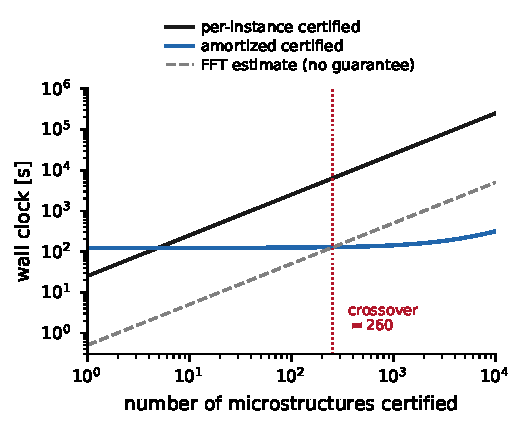
\includegraphics[width=\linewidth]{figures/fig_amortization.pdf}
\caption{Cost to a certified answer. The amortized route overtakes repeated per-instance certification immediately and repeated FFT solves at roughly 300 microstructures, while returning an interval rather than an estimate.}
\label{fig:amortization}
\end{figure}


\begin{figure}[t]
\centering
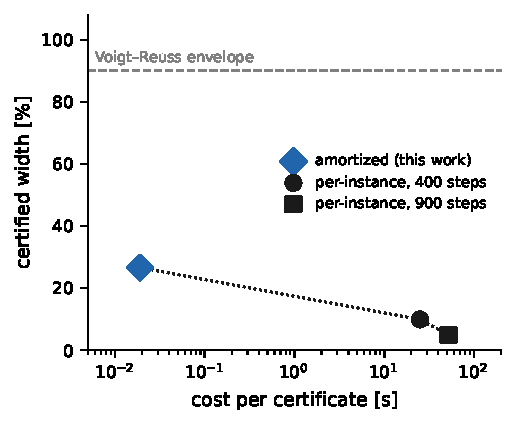
\includegraphics[width=0.62\linewidth]{figures/fig_tightness_cost.pdf}
\caption{Certified width against cost per certificate. Per-instance
training buys tightness at three orders of magnitude more cost per
microstructure; both routes remain far inside the Voigt--Reuss envelope.
A practitioner may choose either, and the amortized route is intended for
screening rather than final design.}
\label{fig:tightness-cost}
\end{figure}

\subsection{Controlled synthetic plane-strain demonstration}
\label{sec:amortized:elastic}

We next exercise the plane-strain construction on a controlled family of
synthetic periodic two-phase cells. With six displacement heads and three
Airy potentials, an operator trained on $200$ generated microstructures for
$4000$ steps in single precision on one GPU ($878$\,s), and certified in
double precision on the CPU by exact integration, produced intervals for
twelve generated held-out cells with median relative width $28.3\%$ (range
$11.2\%$--$45.5\%) at $62$\,ms per certificate. These values quantify
tightness and amortization within this specified generated family; they are
not an externally labelled elasticity coverage study.

For all twelve cells, the projected fields satisfied the certification
contract and the one-sided internal consistency check
$C_{\mathrm{low}} \preceq C_{\mathrm{FEM}}(h)$ held for a conforming $Q_1$
calculation of the same discretised model. This follows from the nested
admissible spaces and checks the implementation path; it is not an
independent validation of the resulting interval against an external
effective-stiffness reference.

\subsection{External public-data coverage audit}
\label{sec:amortized:external}

We next evaluate coverage against the public two-dimensional plane-strain
portion of DaRUS-5730~\cite{Keshav2026data}. The archive provides periodic
binary $100\times100$ rasters and effective stiffness tensors generated by
the Fourier-Accelerated Nodal Solver under periodic boundary conditions. We
retain the released raster without resampling. The released tensor is in an
engineering-Voigt raster frame, whereas the finite-element calculation uses
a right-handed Cartesian frame. We therefore apply the exact Mandel
coordinate transformation $T=\operatorname{diag}(1,1,-1)$ after the usual
Voigt-to-Mandel conversion. This reverses only the normal--shear couplings;
it is a change of coordinates, not a fit or an alteration of a label.

After resolving this coordinate convention by independent $Q_1$ calculations,
we fixed the scaled protocol: $40$ training cells and $40$ validation cells
were selected from each of five Fourier-mode grids, giving $200$ label-free
training cells and $200$ disjoint labelled validation cells. We trained for
$500$ steps and certified every validation cell on the native
$100\times100$ phase-aligned $Q_1$/BFS mesh. The result is reported in
Table~\ref{tab:external-elasticity}.

\begin{table}[t]
\centering
\caption{Fixed external plane-strain coverage audit on DaRUS-5730. Training
uses no reference stiffness tensor. Margins are the smallest eigenvalues of
$C_{\rm ref}-C_{\rm low}$ and $C_{\rm up}-C_{\rm ref}$ in the common
Cartesian Mandel frame.}
\label{tab:external-elasticity}
\resizebox{\textwidth}{!}{%
\begin{tabular}{lr}
\toprule
quantity & result \\
\midrule
training / held-out cells & $200$ / $200$ \\
native raster and certification mesh & $100\times100$ / $100\times100$ \\
reference containment & $200/200$ (100\%) \\
minimum $\lambda_{\min}(C_{\rm ref}-C_{\rm low})$ & $1.264\times10^{-2}$ \\
minimum $\lambda_{\min}(C_{\rm up}-C_{\rm ref})$ & $3.141$ \\
median certified relative width & $160.9\%$ \\
median Voigt--Reuss-width / certified-width & $1.05\times$ \\
independent periodic $Q_1$ checks & $3$ raw-frame failures from this cohort, max. relative tensor error $8.40\times10^{-11}$ \\
\bottomrule
\end{tabular}}
\end{table}

All $200$ transformed reference tensors lie strictly inside the reported
L\"owner intervals. In contrast, comparing the tensor in its raw raster
frame produces $175/200$ containment; that apparent failure is entirely
explained by the sign of the normal--shear couplings. Independent
matrix-free periodic $Q_1$ calculations on three of the cells that fail in
the raw frame reproduce all components of the transformed reference tensor
to relative error at most $8.40\times10^{-11}$. The external certificates
are wide (median $160.9\%$) and only modestly tighter than the analytic
envelope (median $1.05\times$). Thus this experiment validates the
geometry, material law, coordinate convention and coverage contract; it
does not establish competitive external tightness or predictive accuracy.

We report two negative or unexpected results in the interest of an honest
record.

\paragraph{The limit is capacity, not compute.} The monitored gap fell from
$75.4\%$ to $25.3\%$ by step $1200$ and then remained flat through step
$4000$; a smaller run using $40$ microstructures and $450$ steps reached a
held-out median of $28.2\%$, statistically indistinguishable from the
$28.3\%$ obtained with five times the data and nine times the steps.
Table~\ref{tab:ablation} identifies the cause. Network width and depth both
improve the certificate monotonically, whereas tripling the number of
conditioning modes does not help at all. The plateaued configuration sat
mid-range in both width and depth, so additional optimisation could not
help: the model was capacity-saturated rather than under-trained. We note a
practical constraint surfaced by the sweep, that the conditioner
requires $k_{\max} < n/2$ for an $n$-pixel microstructure, so coarse
geometries cap conditioning richness independently of the network.

\begin{table}[t]
\centering
\caption{Architecture ablation at fixed budget (elasticity, 14
microstructures, $150$ steps). Width and depth help; conditioner richness,
tested separately on $16$-pixel geometries where higher modes are
representable, does not.}
\label{tab:ablation}
\resizebox{\textwidth}{!}{%
\begin{tabular}{llrr}
\toprule
sweep & setting & parameters & median width \\
\midrule
width (depth 3) & 32 & 5{,}609 & 35.7\% \\
                & 64 & 19{,}401 & 34.5\% \\
                & 96 & 41{,}385 & \textbf{31.8\%} \\
\midrule
depth (width 64) & 2 & 11{,}081 & 35.2\% \\
                 & 3 & 19{,}401 & 34.5\% \\
                 & 4 & 27{,}721 & \textbf{32.6\%} \\
\midrule
conditioner $k_{\max}$ & 3 (27 modes) & --- & \textbf{25.1\%} \\
                       & 6 (90 modes) & --- & 26.5\% \\
\bottomrule
\end{tabular}}
\end{table}

\paragraph{Amortization stabilises training.} Three independently seeded
operators trained on the same family agreed to within $0.3$ percentage
points of median width ($36.5\%$, $36.7\%$, $36.4\%$ at a reduced budget),
with all fifteen held-out certificates valid. This contrasts sharply with
per-instance training, where at identical settings four seeds produced
certified widths between $0.4\%$ and $1.7\%$ and a fifth collapsed to
$97.8\%$ (Section~\ref{sec:quad:gate}). We attribute the difference to
averaging: the amortized objective sums over many microstructures, so no
single instance can drive the network into the degenerate high-bandwidth
configuration that produces a collapse, whereas the per-instance objective
offers no such regularisation. Stability, not only cost, is therefore a
consequence of amortization, and one that a per-instance formulation
cannot obtain.

\subsection{Screening: what a wide certificate decides}
\label{sec:amortized:screening}

A certified interval of $28\%$ may appear too wide to support a decision.
It is not, because a requirement falling outside the interval decides the
candidate provably. Screening a pool of $40$ unseen microstructures against
a required effective conductivity, at $10$\,ms per candidate:

\begin{table}[t]
\centering
\caption{Provable screening decisions from amortized certificates. PASS
means the certified lower bound already meets the requirement; FAIL that
the upper bound cannot. The last column counts decisions contradicted by an
independent finite-volume reference.}
\label{tab:screening}
\resizebox{\textwidth}{!}{%
\begin{tabular}{rrrrrr}
\toprule
requirement & PASS & FAIL & undecided & decided & wrong \\
\midrule
1.6 & 25 & \phantom{0}2 & 13 & 68\% & 0 \\
1.8 & 17 & \phantom{0}8 & 15 & 62\% & 0 \\
2.0 & 11 & 14 & 15 & 62\% & 0 \\
2.2 & 10 & 16 & 14 & 65\% & 0 \\
2.4 & \phantom{0}6 & 19 & 15 & 62\% & 0 \\
\bottomrule
\end{tabular}}

\end{table}

Between $62\%$ and $68\%$ of the pool is decided provably and no decision
is contradicted by the reference, as must be so, since the decisions
follow from bounds that provably contain the truth. The remainder is not a
failure but an honest referral to per-instance certification, which reaches
widths below $1\%$. A point-estimate surrogate, however accurate, can rank
candidates but cannot prove one acceptable.

\subsection{When amortization pays}
\label{sec:amortized:crossover}

Amortization is not a speed claim against classical solvers. A
Moulinec--Suquet FFT solve of these cells takes of order $1$\,s, roughly
fifty times faster than a per-instance certified solve, and we make no
contrary claim. The relevant comparison is many-query cost against a
\emph{certified} answer: with $123$\,s of training and $19$\,ms per
certificate, the amortized route overtakes repeated per-instance
certification at approximately $300$ designs, and thereafter by a widening
margin. What the FFT solve does not provide, at any cost, is a two-sided
interval that provably contains the effective tensor; the certified
interval is the object being amortized, and its value is assessed in
Section~\ref{sec:tightness}.
